
\section{Placement}
\label{sec:placement}
So far we have only dealt with the technology where we consider the problem space and adress the constraints of the hardware architecture. 
For every constraint, we devise a solution to fully address it or a simplification that sacrifices some optimization but reduces the complexity of the problem space. 

Now that we have dealt with the bulk of these constraints and squared them away into self-contained \texttt{SiteInst}s, we can now apply some general optimization algorithms to finally address our optimization objective, which is to place these \texttt{SiteInst} objects onto the device while minimizing wirelength. 

\subsection{Simulated Annealing}
\label{subsec:simulated_annealing}

In this paper we implement and present a basic Simulating Annealing (SA) placer. 
As mentioned in the Introduction, SA is a metaheuristic that approximates a global optimum in a large optimization search space. 
Its name is borrowed from metallurgy and is inspired by the physical process of heating a metal and then slowly lowering the temperature to decrease structural atomic defects, thus minimizing the system energy. 
SA does not guarantee a globally optimal solution, but provides solutions that are often "good enough", especially when an approximate global optimum is more important than finding a precise local optimum in a fixed amount of time. 
SA is typically employed in discrete combinatorial optimization problems like the travelling salesman problem or job-shop scheduling. 

The state \texttt{s} of the system and the function \texttt{E(s)} to be minimized is analogous to the internal energy of the system. 
The goal of SA is to bring the system from some initial state to a state with the minimum possible energy until an energy budget met or until a computational budget is exceeded.
At each step or iteration, the SA heuristic considers some neighboring state \(s^*\). 
If \(s^*\) has a lower energy than \(s\), then the state transition from \(s\) to \(s^*\) is accepted outright.
If \(s^*\) has a higher energy, then it can be probabilistically accepted depending on the current global temperature.
The global temperature starts at some positive amount then gradually decreases to zero according to a cooling schedule, which can be linear, geometric, logarithmic, or some piecewise combination. 
The higher the temperature, the higher the likelihood of accepting an energy-increasing move. 
The selection of cooling schedule parameters is usually fine tuned after empirical experimentation. 

%
%
%
%

In the context of our placer, we use SA to minimize wirelength between \texttt{SiteInst}s when placed over the discrete \texttt{Site}s of the FPGA \texttt{device}.
The state \texttt{s}
In each iteration of the SA algorithm, a new 

%
%
%
%

Shown in Listing \ref{lst:sa_outer} is a simplified pseudocode for the outer-most loop of the SA algorithm. 
First, we unplace all of the SiteInsts and then randomly place them across the device.
Then, we enter the outer-most loop which terminates when the number of passes exceeds a maximum amount, in this case, 300 passes. 
In each pass, we move() the design, then update the global temperature. 

In each or move() or "pass", we iterate through every single \texttt{SiteInst} and \texttt{SiteInst} chain, propose a move to a new placement. 
If the proposed \texttt{Site} is already occupied by a resident \texttt{SiteInst}, we evaluate a swap. 
Each move or swap is evaluated by calculating the HPWL cost before and after the movement.
If the move reduces the HPWL cost, then the movement is accepted outright.
If the move increases cost, then it can be accepted by chance depending on if the global temperature is high enough to permit the hill-climb.

\begin{lstlisting}[language=java, caption={SA pseudocode: outer loop}, label={lst:sa_outer}]
public void placeDesign(PackedDesign packedDesign) {
    // unplace the pseudorandom packed placement
    unplaceAllSiteInsts(packedDesign);
    // place randomly
    randomInitialPlacement(packedDesign);
    int passes = 0;
    while (passes < 300) {
        updateTemperature(passes);
        move(packedDesign)
        passes++;
    }
}

private void move(PackedDesign packedDesign) {
    moveSiteChains(packedDesign.DSPSiteInstCascades);
    moveSiteChains(packedDesign.CARRYSiteInstChains);
    moveSingleSite(packedDesign.RAMSiteInsts);
    moveSingleSite(packedDesign.CLBSiteInsts);
}
\end{lstlisting}

\newcolumn
\begin{lstlisting}[language=java, caption={Single Site Movement}, label={lst:sa_move_single}]
protected void moveSingleSite(List<SiteInst> sites) {
for (SiteInst si : sites) {
    SiteTypeEnum ste = si.getSiteTypeEnum();
    List<Site> homeConns = findConnectedSites(si, null);
    Site homeSite = si.getSite();
    Site awaySite = proposeSite(si, homeConns, true);
    SiteInst awaySi = occupiedSites.get(ste).get(awaySite);
    double oldCost = 0;
    double newCost = 0;
    if (awaySi != null) {
        List<Site> awayConns = findConnectedSites(awaySi, null);
        oldCost += evaluateSite(homeConns, homeSite);
        oldCost += evaluateSite(awayConns, awaySite);
        newCost += evaluateSite(homeConns, awaySite);
        newCost += evaluateSite(awayConns, homeSite);
    } else {
        oldCost += evaluateSite(homeConns, homeSite);
        newCost += evaluateSite(homeConns, awaySite);
    }
    if (evaluateMoveAcceptance(oldCost, newCost)) {
        if (awaySi != null) {
            unplaceSiteInst(si);
            unplaceSiteInst(awaySi);
            placeSiteInst(si, awaySite);
            placeSiteInst(awaySi, homeSite);
        } else {
            unplaceSiteInst(si);
            placeSiteInst(si, awaySite);
        }
    }
}
} // end randomMoveSingleSite()
\end{lstlisting}

\begin{lstlisting}[language=java, caption={Move Acceptance with Temperature}, label={lst:sa_acceptance}]
protected boolean evaluateMoveAcceptance(double oldCost, double newCost) {
    // if the new cost is lower, accept it outright
    if (newCost < oldCost)
        return true;
    // otherwise, evaluate probability to accept higher cost
    double delta = newCost - oldCost;
    double acceptanceProbability = 
        Math.exp(-delta / this.currentTemp);
    return Math.random() < acceptanceProbability;
}
\end{lstlisting}


{
    \centering
    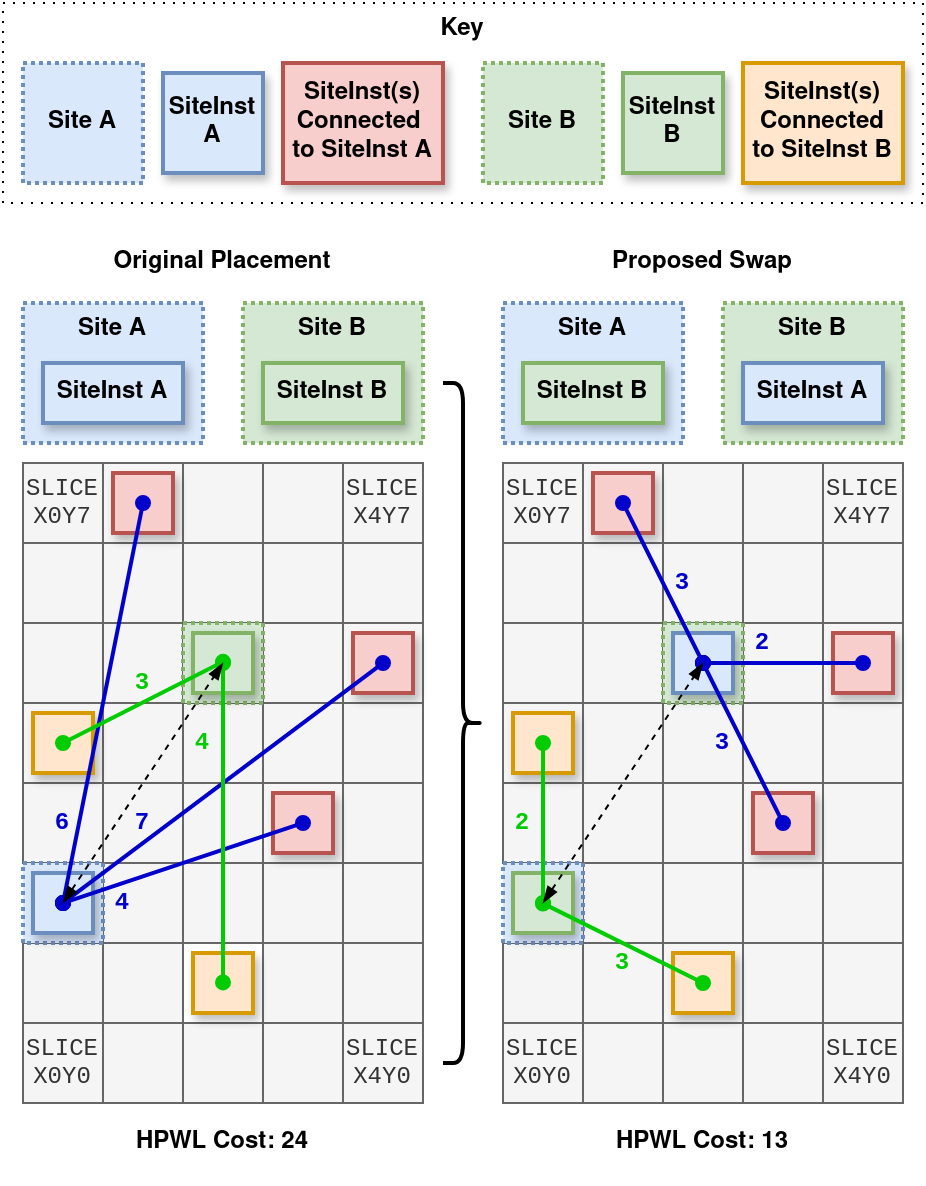
\includegraphics[width=\columnwidth]{figures/placement/swapSingleSite.png}
    \captionof{figure}{Single Site Swap Proposal}
    \label{fig:swapSingleSite}
}

% \begin{lstlisting}[language=java, caption={Chain Swapping}, label={lst:chain_swap_pseudocode}]
% protected void moveSiteChains(List<List<SiteInst>> chains) {
% for (List<SiteInst> current_chain : chains) {
%     /*
% 
%     1) Draw a vertical window of equal size to the current chain. We will refer to this window as the "home window". 
%     2) Select a new candidate anchor for this chain.
%     3) Project the home window onto the candidate anchor with anchors coinciding. We will refer to this projected window as the "away window".
%     4) Check if there are any resident SiteInsts or SiteInst chains present in the away window. Check if the away window breaks any resident SiteInst chains. 
%     5)  IF (the away window breaks any chains): 
%             extend the window in either direction to 
%             fully accommodate all resident chains. 
%         ELSE: GOTO evaluateMove(). 
%     6) Project the extended away window back onto the original region with the tail of the window coinciding with the tail of the current chain. This projected window becomes the new home window. 
%     7) WHILE (the home window breaks any resident chains):
%         shift the window upwards by one Site. 
%         IF (num_shifts > home_win_size - current_chain.size()):
%             reject the candidate swap.
%             CONTINUE onto next chain
%     8) int oldCost = evaluateCost(original placement) 
%     9) int newCost = evaluateCost(proposed placement) 
%     10) evaluateMoveAcceptance(oldCost, newCost, temperature) 
%     11) IF (move accepted):
%             element-wise swap SiteInsts in both windows
% 
%     */
% }
% }
% \end{lstlisting}

\newcolumn
\begin{lstlisting}[language=Java, caption={Chain Swapping Pseudocode}, label={lst:chain_swap_pseudocode}]
protected void moveSiteChains(List<List<SiteInst>> chains) {
for (List<SiteInst> currentChain : chains) {
    int chainSize = currentChain.size();

    // Step 1: Identify home window for this chain
    Site homeAnchor = currentChain.get(0).getSite();
    List<Site> homeWindow = getSitesInWindow(homeAnchor, chainSize);

    // Step 2: Select a candidate away anchor
    Site awayAnchor = proposeAnchorSite(currentChain, homeWindow, true);

    // Step 3: Determine away window based on awayAnchor and chainSize
    List<Site> awayWindow = getSitesInWindow(awayAnchor, chainSize);

    // Step 4: Find any resident SiteInst chains in the away window
    List<List<SiteInst>> residentChainsInAway = 
        collectChainsInWindow(siteType, awayWindow);

    // Step 5: If any resident chains overlap, extend the away window to include them
    if (!residentChainsInAway.isEmpty()) {
        awayWindow = extendWindowToIncludeChains(awayWindow, residentChainsInAway);
    }

    // Step 6: Map the (possibly extended) away window back onto the original region 
    //         so that the tail of that window coincides with the tail of the current chain
    List<Site> candidateHomeWindow = mapAwayToHomeWindow(
        homeAnchor, awayWindow, chainSize);

    // Step 7: While the candidate home window still overlaps resident chains, shift upward
    int shifts = 0;
    while (windowHasOverlap(candidateHomeWindow)) {
        candidateHomeWindow = shiftWindowUp(candidateHomeWindow);
        shifts++;
        if (shifts > (homeWindow.size() - chainSize)) {
            // Reject this swap attempt and move on to the next chain
            continue;
        }
    }

    // Step 8: Compute cost of the original placement in home window
    double oldCost = evaluateWindowCost(homeWindow);

    // Step 9: Compute cost of the proposed swap placement
    double newCost = evaluateWindowCostForSwap(
        homeWindow, awayWindow, currentChain);

    // Step 10: Decide whether to accept the move based on oldCost, newCost, and temperature
    if (evaluateMoveAcceptance(oldCost, newCost, currentTemp)) {
        // Step 11: Perform an element-wise swap of SiteInsts between homeWindow and awayWindow
        swapChainsBetweenWindows(homeWindow, awayWindow);
    }
}
}
\end{lstlisting}

\newpage
\end{multicols}
{
    \centering
    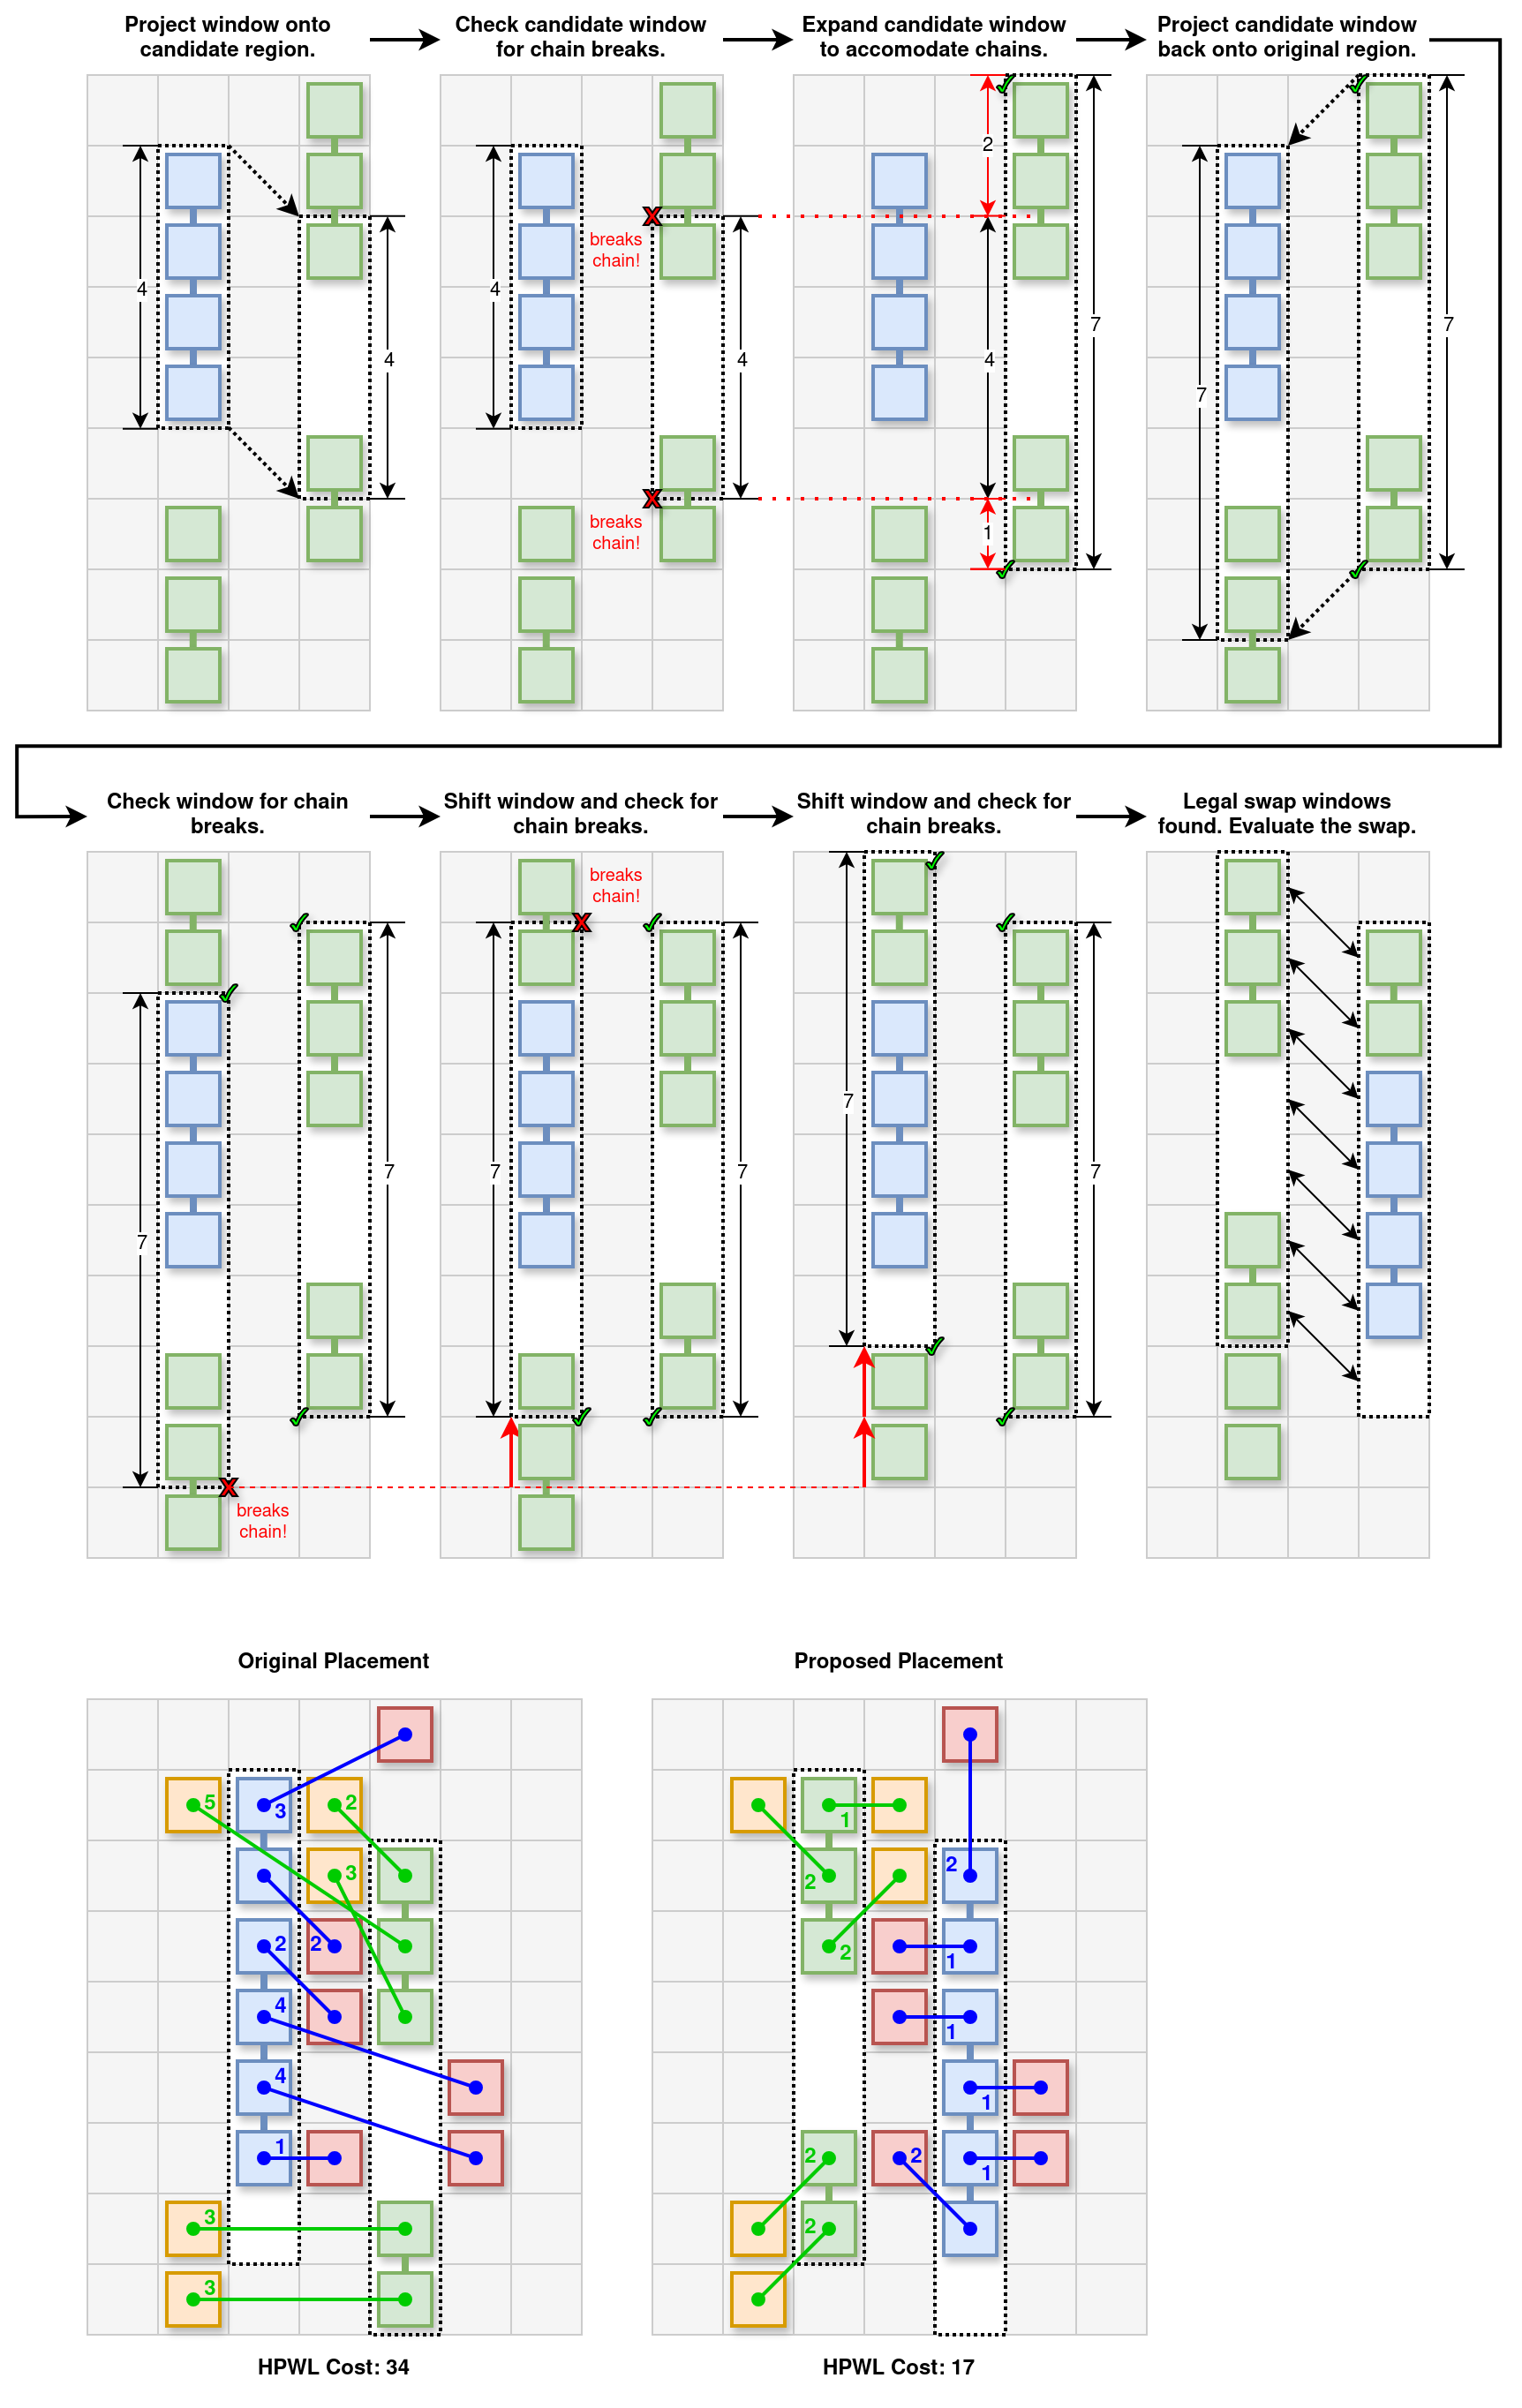
\includegraphics[width=0.9\columnwidth]{figures/placement/swapSiteChain.png}
    \captionof{figure}{Site Chain Swap Proposal}
    \label{fig:swapChainSite}
}
\begin{multicols}{2}

Select a new anchor Site.
Project a window onto the proposed Site
If the window anchor breaks a chain, extend the window in its direction until the anchor coincides with the chain anchor..
If the window tail breaks a chain, extend the window in its direction until the tail coincides with the chain tail.



